\section{Exercise 8 - Lab 2}

Yêu cầu: Di chuyển hàm quét LED \texttt{update7SEG()} từ hàm ngắt timer ra ngoài hàm \texttt{()}. Đảm bảo ngắt timer lúc này chỉ được sử dụng duy nhất cho việc xử lý đếm lùi các timer phần mềm. ọi xử lý hoặc tính toán phức tạp phải được đưa vào vòng lặp while trong hàm chính để tối ưu hóa sự phức tạp cho hàm phục vụ ngắt

Ý tưởng: Mở rộng timer phần mềm thành mảng để  nhiều tác vụ đồng thời. Cấp phát timer 0 cho đèn 4 LED 7 đoạn, timer 1 cho DOT và timer 2 cho đèn LED. Tốc độ quét cần được cài đặt ở mức phù hợp. 

\begin{lstlisting}[language=C, caption={Phần code hiện thực}, label={lst:ex6_lab2}]
     updateClockBuffer();
    setTimer(0, 250);  //  LED (250ms)
    setTimer(1, 500);  // DOT (500ms)
    setTimer(2, 1000); //  Clock & LED_RED (1000ms)
    HAL_TIM_Base_Start_IT(&htim2);
  /* USER CODE END 2 */

  /* Infinite loop */
  /* USER CODE BEGIN WHILE */
    while (1)
    {
    /* USER CODE END WHILE */

    /* USER CODE BEGIN 3 */

        if(timer_flag[0] == 1){
            HAL_GPIO_WritePin(GPIOA,GPIO_PIN_6|GPIO_PIN_7|GPIO_PIN_8|GPIO_PIN_9, GPIO_PIN_SET);
            update7SEG(index_led);
            setTimer(0, 250);
        }
        if(timer_flag[1] == 1){
            HAL_GPIO_TogglePin(GPIOA, GPIO_PIN_4);
            setTimer(1, 500);
        }
        if(timer_flag[2] == 1){
            HAL_GPIO_TogglePin(LED_RED_GPIO_Port, LED_RED_Pin);

            second++;
            if(second >= 60) {
                second = 0;
                minute++;
            }
            if(minute >= 60) {
                minute = 0;
                hour++;
            }
            if(hour >= 24) {
                hour = 0;
            }
            updateClockBuffer();
            setTimer(2, 1000);
        }
    }
  /* USER CODE END 3 */


  void HAL_TIM_PeriodElapsedCallback(TIM_HandleTypeDef *htim){
	if(htim->Instance == TIM2){
		timer_run();
	}

}

  
\end{lstlisting}


\begin{figure}[h!]
\begin{center}
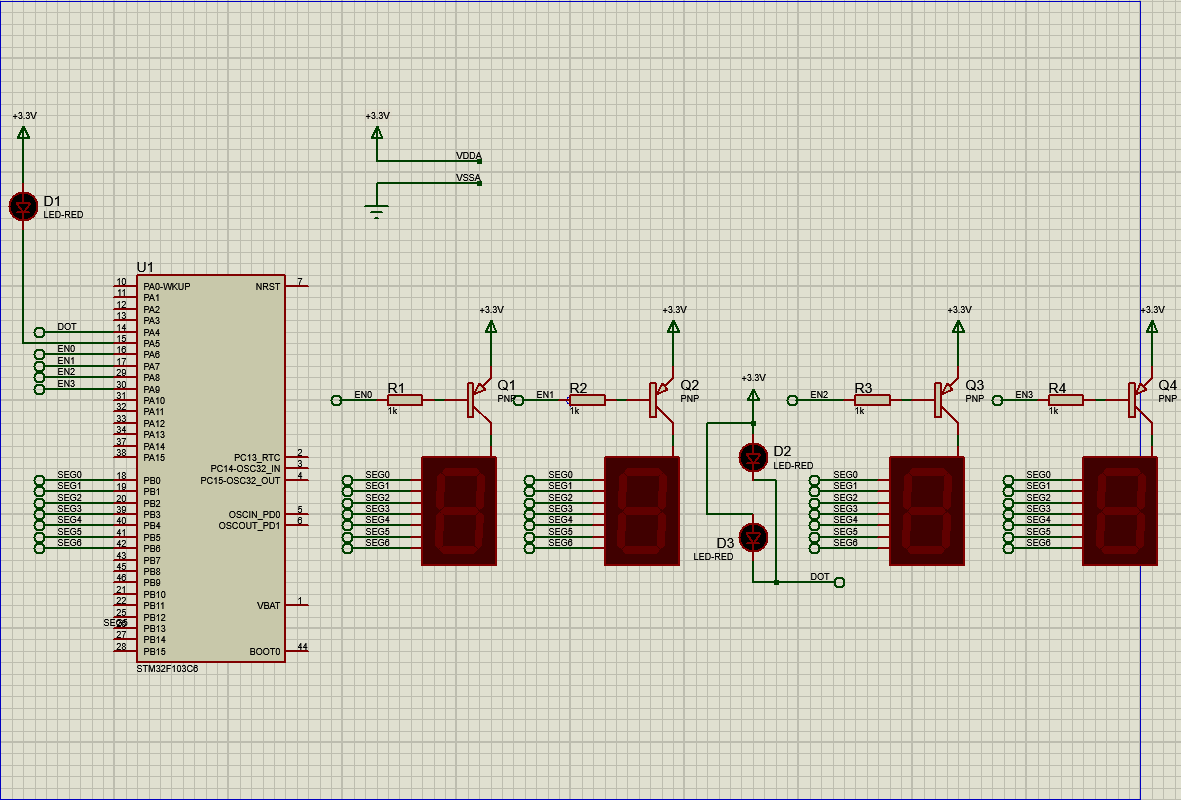
\includegraphics[width=13cm]{Picture/lab2_ex8.png}
\end{center}
\caption{Mô phỏng bài 8}
\label{fig:1}
\end{figure}

